\subsection{Tools > Projection > Unroll}
\label{subsection:unroll}

\begin{figure}[!htb]
\begin{center}
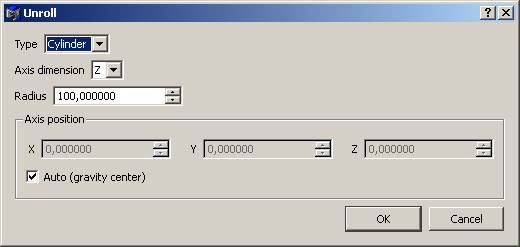
\includegraphics[width=0.6\textwidth]{Partie3_Fonctions/unrollDlg.png}
\caption{\label{fig:unrollDlg}Interface de param�trage pour l'outil de \emph{d�veloppement} d'un nuage}
\end{center}
\end{figure}

\index{developper@d�velopper}
\index{derouler@d�rouler|see{d�velopper}}
Cette fonction permet de \emph{d�velopper} sur un plan un nuage de point consid�r� comme �tant port� par une
forme de r�volution (cylindre ou un cone). Voir figure~\ref{fig:unrollExample}.
\\
\par
Il faut pour cela renseigner diff�rents param�tres d�finissant la forme de r�volution :
\begin{itemize}
\item le type (cylindre ou cone)
\item la dimension selon laquelle est positionn�e l'axe de d�veloppement (X, Y ou Z pour l'instant)
\item un point par lequel passe cet axe (dans le cas o� la checkbox \emph{auto axis} est s�lectionn�e, ce point est automatiquement
remplac� par le centre de gravit� du nuage)
\item le rayon du cylindre ou la base du cone
\item et l'angle d'ouverture du cone le cas �ch�ant\\
\end{itemize}
\par
\textcolor[rgb]{1.00,0.00,0.00}{Attention, pour optimiser la m�moire, cette fonction applique la transform�e
directement sur l'entit� s�lectionn�e ! Il peut �tre n�cessaire d'utiliser avant l'outil de clonage\index{cloner} -
voir section~\ref{subsection:clone}.}

\begin{figure}[!htb]
\begin{center}
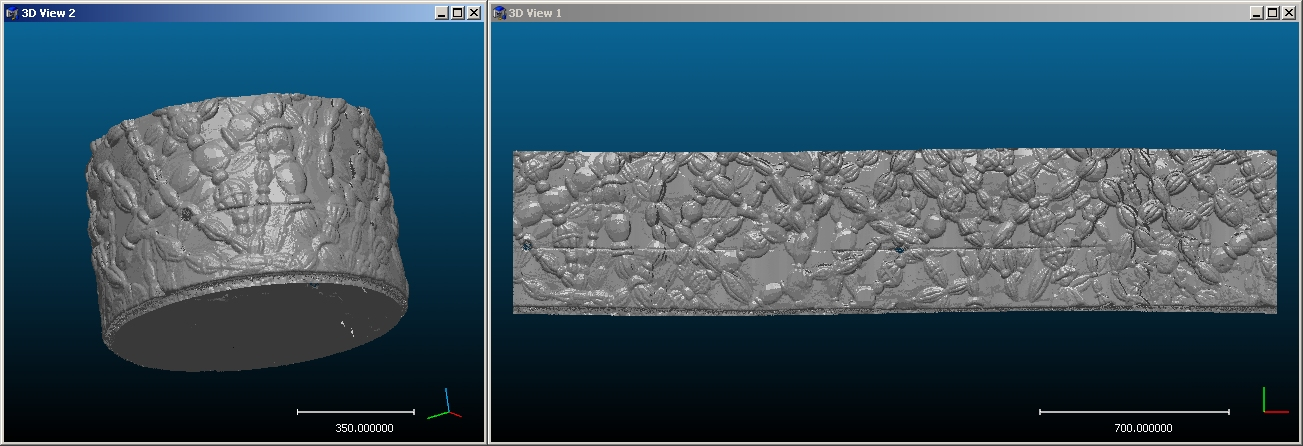
\includegraphics[width=0.9\textwidth]{Partie3_Fonctions/unroll.jpg}
\caption{\label{fig:unrollExample}Exemple de r�sultat : nuage de points cylindrique (� gauche), et sa d�velopp�e
(� droite)}
\end{center}
\end{figure}
